\documentclass[pdf,aspectratio=169]{beamer}
\usepackage[]{hyperref,graphicx,siunitx,booktabs,lmodern}
\usepackage{physics}
\usepackage{em-commands}
\usepgfplotslibrary{statistics}
\mode<presentation>{\usetheme{EM}}

%Question Numbering
\newcounter{questionnumber}
\newcommand{\qnum}{%
	\stepcounter{questionnumber}%
	Q\arabic{questionnumber}
}
\resetcounteronoverlays{questionnumber}

\graphicspath{ {../Images/} }

\sisetup{per-mode=symbol}

\tikzstyle{plate}=[draw, very thick, minimum width=4cm, minimum height=1cm, fill=gray!40, anchor=south]

%preamble
\title{}
\date{October 17, 2018}
\author{Jed Rembold}

\begin{document}
\renewcommand{\theenumi}{\Alph{enumi}}

\begin{frame}{Announcements}
	\begin{itemize}
		\item Congrats to Ricky for making the best maze solver last Thursday!
			\begin{itemize}
				\item And congrats to Cassie for being the bold person to solve a large one by hand!
				\item You can still get in on the fun at \url{http://jrembold.github.io/code_challenge}
			\end{itemize}
		\item Exam 1 is getting handed back!
			\begin{itemize}
				\item You can add 1 to your score
			\end{itemize}
		\item Homework 7 is due tonight!
		\item Starting Chapter 5 on Wednesday. Read 5.1
	\end{itemize}
\end{frame}

\begin{frame}{Test Results}
  \begin{columns}
	\column{.7\textwidth}
	  \begin{figure}[h!]
		\centering
		\begin{tikzpicture}
		  \begin{axis}[
			width=10cm,
			height=7cm,
			xlabel= Percentage,
			ylabel= Number of Students,
			yticklabels={,,},
			ylabel near ticks,
			xmin = 60, xmax=100,
		  ]
		  \addplot [hist={bins=6}, fill=red!75!black ] table[y=Percentage, col sep=comma] {Exam1_Scores.csv};
		  \end{axis}
		\end{tikzpicture}
	  \end{figure}
	  \column{.3\textwidth}
	  \begin{itemize}
		\item High: 96\%
		\item Mean: 80\%
		\item Median: 81\%
	  \end{itemize}
	\end{columns}
\end{frame}

\begin{frame}{Question 1 \hspace{10cm}55\%}
	For the below symmetric charge distribution, what $r$ dependence would the \emph{electric field} have far from the charges?
	\begin{center}
		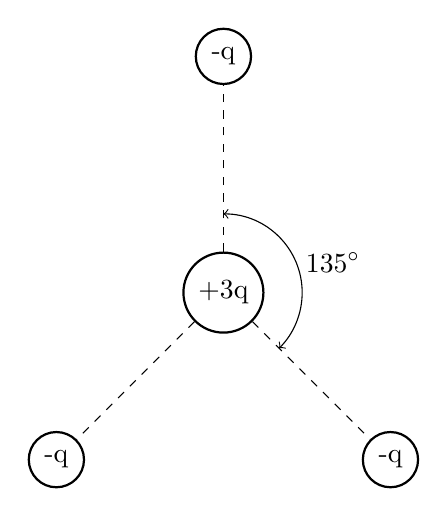
\begin{tikzpicture}
			\node[draw, thick, circle](p) at (0,0) {+3q};
			\node[draw, thick, circle](n1) at (0,3) {-q};
			\node[draw, thick, circle](n2) at (-45:3) {-q};
			\node[draw, thick, circle](n3) at (225:3) {-q};
			\path[dashed] (p) edge (n1) (p) edge (n2) (p) edge (n3);
			\draw[<->] (0,1) arc (90:-45:1) node[midway,right] {\ang{135}};
		\end{tikzpicture}
	\end{center}
\end{frame}

\begin{frame}{Question 2 \hspace{10cm}72.5\%}
	What is the total energy contained in the below system of charges?
	\begin{center}
		\begin{tikzpicture}
			\node[draw, thick, circle] (1) at (0,0) {$+q$};
			\node[draw, thick, circle] (2) at (0:3) {$-q$};
			\node[draw, thick, circle] (3) at (60:3) {$+q$};
			\draw[dashed]
				(1) -- (2) node[midway,below,math] {r_0}
				(1) -- (3) node[midway,above,sloped,math] {r_0}
				(3) -- (2) node[midway,above,sloped,math] {r_0};
		\end{tikzpicture}
	\end{center}
\end{frame}

\begin{frame}{Question 3 \hspace{10cm} 53.7\%}
	Write down an expression for the volume charge density, $\rho(\pos)$, of a system containing all of the following:
	\begin{itemize}
		\item A charge of $+2q$ located at $\pos=(2,2,0)$
		\item A charge of $-q$ located at $\pos=(5,0,2)$
		\item A line charge with density $\lambda_0$ which extends infinitely in the $\yhat$ direction and passes through the point $\pos=(-1,0,-3)$.
	\end{itemize}
\end{frame}

\begin{frame}{Question 4 \hspace{10cm} 79\%}
	Can the vector field below have a consistent corresponding ``potential'' defined? Why or why not?
	\begin{center}
		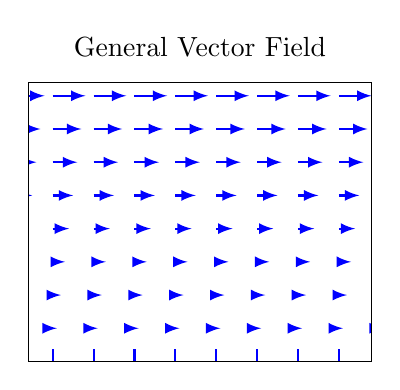
\begin{tikzpicture}
			\begin{axis}[
				domain=0:1,
				view={0}{90},
				samples=15,
				title=General Vector Field,
				xmin=0.1, xmax=.7,
				ymin=0, ymax=.6,
				width=.49\textwidth,
				ticks=none,
				]
				\addplot3[blue, quiver={
						u={y},
						v={0},
						scale arrows=0.1,
					},
					-latex, thick,
					] (x,y,0);
			\end{axis}
		\end{tikzpicture}
	\end{center}
\end{frame}

\begin{frame}{Question 5 \hspace{10cm}82\%}
	A large rectangular pipe has charge spread along the exterior that drives a uniform electric field through the pipe as shown. In the middle of the pipe lies a sheet (insulated from the sidewalls). To the left of the sheet the electric field has a magnitude of $E_0$, to the right of the sheet the magnitude of the electric field is $\tfrac{E_0}{2}$. What is the surface charge density of the sheet in the center (far from the sidewalls)? What overall concept did you employ to find your answer?
	\begin{center}
		\begin{tikzpicture}
			\draw[thick]
				(0,0,0) -- +(10,0,0)
				(0,2,0) -- +(10,0,0)
				(0,0,2) -- +(10,0,0);
			\draw[very thick, fill=gray!50, line join=round]
				(5,0,0) -- (5,2,0) -- (5,2,2) -- (5,0,2) -- cycle;
			\draw[thick]
				(0,2,2) -- +(10,0,0);
			\draw[ultra thick, -latex] (1,1,1) -- +(1,0,0) node[right,math] {\ef=E_0 \yhat};
			\draw[ultra thick, -latex] (6,1,1) -- +(1,0,0) node[right,math] {\ef=\tfrac{1}{2}E_0 \yhat};
		\end{tikzpicture}
	\end{center}
\end{frame}

\begin{frame}{Question 6 \hspace{10cm} 68\%}
	An electric field is described by:
	\[\ef = E_0\left(3y\xhat + \left(3x - 2y\sin(z)\right)\yhat - y^2\cos(z)\zhat\right)\]
	What is the potential difference when moving from the point $\pos_1 = 4\xhat + 2\yhat$ to $\pos_2= 6\xhat + 2\yhat + \pi\zhat$?
\end{frame}

\begin{frame}{Question 7 \hspace{10cm} 88.6\%}
	The general solution for spherical separation of variables is
	\[V(r,\theta) = \sum_{\ell=0}^\infty \left(A_\ell r^\ell + \frac{B_\ell}{r^{\ell+1}}\right)P_\ell(\cos\theta)\]
	Given that the potential on the surface of a sphere is given by:
	\[V(R,\theta) = V_0\left(3\cos^2\theta + 4\cos\theta - 1\right)\]
	Write down the final solution of the potential inside the sphere. (\emph{Your answer should only depend on constants and $r$ and $\theta$, not in terms of Legendre polynomials.})
\end{frame}

\begin{frame}{\qnum}
	A point charge $+q$ is placed at the center of a neutral, linear homogeneous dielectric teflon spherical shell. Can $\ed$ be computed from its divergence?
	\[\oint \ed\vdot d\vA = Q_{free}\]
	\vspace*{-1.5cm}
	\begin{columns}
		\column{0.5\textwidth}
		\begin{center}
			\begin{tikzpicture}
				\node[pcharge] at (0,0) {$+q$};
				\draw[fill=orange!40, even odd rule] (0,0) circle (2) circle (3);
			\end{tikzpicture}
		\end{center}
		\column{0.5\textwidth}
		\begin{enumerate}
			\item \alert<2>{Yes}
			\item No
			\item Depends on information not given
		\end{enumerate}
	\end{columns}
\end{frame}

\begin{frame}{\qnum}
	A point charge $+q$ is placed at the center of a neutral, linear, homogeneous, dielectric hemispherical shell. Can $\ed$ be computed from its divergence?
	\begin{columns}
		\column{0.5\textwidth}
		\begin{center}
			\begin{tikzpicture}
				\node[pcharge] at (0,0) {$+q$};
				\draw[fill=orange!40] (-2,0) arc (180:0:2) -- ++(1,0) arc(0:180:3) -- cycle;
			\end{tikzpicture}
		\end{center}
		\column{0.5\textwidth}
		\begin{enumerate}
			\item Yes
			\item \alert<2>{No}
			\item Depends on information not given
		\end{enumerate}
	\end{columns}
\end{frame}

\begin{frame}{\qnum}
	Suppose you have two large conducting plates which have some potential difference $\Delta V$ applied between them. In the region between the plates, you have inserted \emph{two} different dielectrics. When you go to solve Laplace's equation for the region between the plates, how many different boundary conditions do you have?
	\begin{columns}
		\column{0.3\textwidth}
		\begin{enumerate}
			\item 2
			\item 3
			\item \alert<2>{4}
			\item 6
		\end{enumerate}
		\column{0.5\textwidth}
		\begin{center}
			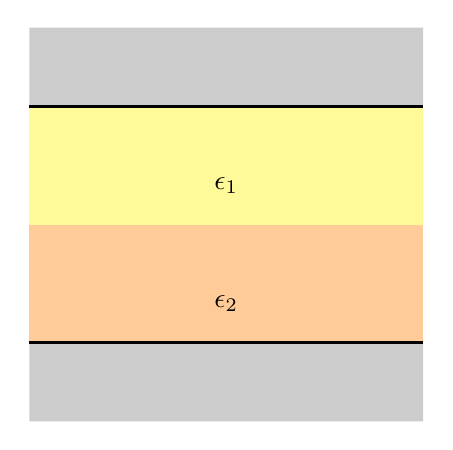
\begin{tikzpicture}
				\fill[gray!40]
					(0,0) rectangle +(5,1)
					(0,4) rectangle +(5,1);
				\fill[orange!40]
					(0,1) rectangle +(5,1.5);
				\fill[yellow!40]
					(0,2.5) rectangle +(5,1.5);
				\draw[very thick]
					(0,1) -- +(5,0)
					(0,4) -- +(5,0);
				\node at (2.5,3) {$\epsilon_1$};
				\node at (2.5,1.5) {$\epsilon_2$};
			\end{tikzpicture}
		\end{center}
		
	\end{columns}
\end{frame}










\end{document}
